\documentclass[hide notes,intlimits,usenames,dvipsnames]{beamer}

\mode<presentation>
{
  \usetheme{Singapore}
  \usefonttheme{professionalfonts}
  \setbeamertemplate{blocks}[rounded][shadow=true]
  \setbeamercovered{transparent}
  \setbeamertemplate{footline}[frame number]
}

% load packages
\usepackage[english]{babel}
\usepackage[latin1]{inputenc}
\usepackage[T1]{fontenc}
\usepackage{lmodern}
\usepackage[multidot]{grffile}
\usepackage{verbatim,empheq}

\usepackage{tikz}
\usetikzlibrary{shapes,arrows,shadows}
\usetikzlibrary{decorations.pathreplacing}

\usepackage{animate}
\usepackage{amsmath,verbatim}

% see http://tex.stackexchange.com/questions/86188/labelling-with-arrows-in-an-automated-way

\newif\ifclipme\clipmetrue
\tikzset{labelstyle/.style={LabelStyle/.append style={#1}},linestyle/.style={LineStyle/.append style={#1}}}
\tikzset{LabelStyle/.initial={},LineStyle/.initial={}}

\newcommand{\mathWithDescription}[4][]{{%
    \tikzset{#1}%
    \tikz[baseline]{
        \node[draw=red,rounded corners,anchor=base] (m#4) {$\displaystyle#2$};
        \ifclipme\begin{pgfinterruptboundingbox}\fi
            \node[above of=m#4,font=\strut, LabelStyle] (l#4) {#3};
            \draw[-,red, LineStyle] (l#4) to (m#4);
        \ifclipme\end{pgfinterruptboundingbox}\fi
    }%
}}

\newcommand{\mathWithDescriptionStarred}[3][]{{%
    \clipmefalse%
    \mathWithDescription[#1]{#2}{#3}{\themathLabelNode}%
}}

\newcounter{mathLabelNode}

\newcommand{\mathLabelBox}[3][]{%
   \stepcounter{mathLabelNode}%
   \mathWithDescription[#1]{#2}{#3}{\themathLabelNode}%
   \vphantom{\mathWithDescriptionStarred[#1]{#2}{#3}{\themathLabelNode}}%
}

\definecolor{dark red}{HTML}{E41A1C}
\definecolor{dark green}{HTML}{4DAF4A}
\definecolor{dark violet}{HTML}{984EA3}
\definecolor{dark blue}{HTML}{084594}
\definecolor{dark orange}{HTML}{FF7F00}
\definecolor{light blue}{HTML}{377EB8}
\definecolor{light red}{HTML}{FB9A99}
\definecolor{light violet}{HTML}{CAB2D6}

\newcommand{\CC}{\mathbb{C}}
\newcommand{\NN}{\mathbb{N}}
\newcommand{\RR}{\mathbb{R}}
\newcommand{\ZZ}{\mathbb{Z}}

\newcommand{\Kcal}{\mathcal{K}}
\newcommand{\Xcal}{\mathcal{X}}

\newcommand{\bF}{\mathbf{F}}
\newcommand{\bQ}{\mathbf{Q}}
\newcommand{\bU}{\mathbf{U}}
\newcommand{\bX}{\mathbf{X}}

\newcommand{\bq}{\mathbf{q}}
\newcommand{\bu}{\mathbf{u}}
\newcommand{\bv}{\mathbf{v}}
\newcommand{\bx}{\mathbf{x}}

\newcommand{\Div}{\nabla\cdot}
\newcommand{\eps}{\epsilon}
\newcommand{\grad}{\nabla}
\newcommand{\lap}{\triangle}
\renewcommand{\bar}{\overline}

\newcommand{\ip}[2]{\ensuremath{\left<#1,#2\right>}}


\newenvironment{transbox}[1][]{%
\begin{tikzpicture}
\node[drop shadow,rounded corners,text width=\textwidth,fill=white, fill opacity=#1,text opacity=1] \bgroup
}{
\egroup;\end{tikzpicture}}


\title[Implicit time-stepping for ice sheets]{Implicit time-stepping for ice sheets}

\author[Bueler]{Ed Bueler}

\institute[UAF]{
  \scriptsize Dept of Mathematics and Statistics and Geophysical Institute \\

  University of Alaska Fairbanks
}

\titlegraphic{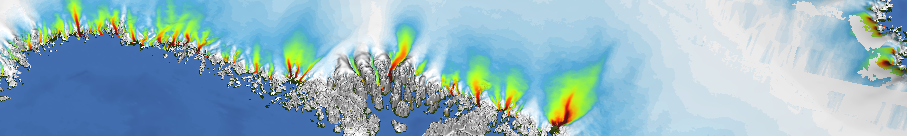
\includegraphics[width=\textwidth]{andycoast.png}}

\beamertemplatenavigationsymbolsempty   % remove faint and silly navigation symbols at bottom
\renewcommand{\insertnavigation}[1]{}   % remove section headings from top of each slide

\setbeamerfont{date}{size=\scriptsize}
\date{}

%\AtBeginSection[]
%{
%  \begin{frame}<beamer>
%    \frametitle{Outline}
%    %\tableofcontents[currentsection,hideallsubsections]
%    \tableofcontents[currentsection]
%  \end{frame}
%}


\begin{document}

\graphicspath{{../../old/commonfigs/}}

\begin{frame}
\vspace{10mm}
  \titlepage
  \begin{center}
  \tiny SIAM CSE \quad 2 March, 2017 \hfill  supported by NASA grant \# NNX13AM16G
  \end{center}
\end{frame}

  \begin{frame}
    \frametitle{Outline}
    \tableofcontents
  \end{frame}

\section{problem, goals, and models}

\begin{frame}{ice sheet flows and their boundaries}
\begin{columns}
\begin{column}{0.45\textwidth}
\begin{itemize}
\item<1> nearly-fractal free boundaries
    \begin{itemize}
    \scriptsize
    \item[$\circ$] location determined by flow, topography, and atmosphere/ocean inputs
    \normalsize
    \end{itemize}
\item<2> large fraction of the boundary: grounded margins
\item<3> surface slope is discontinuous at grounded margins
\end{itemize}
\end{column}
\begin{column}{0.55\textwidth}
\only<1>{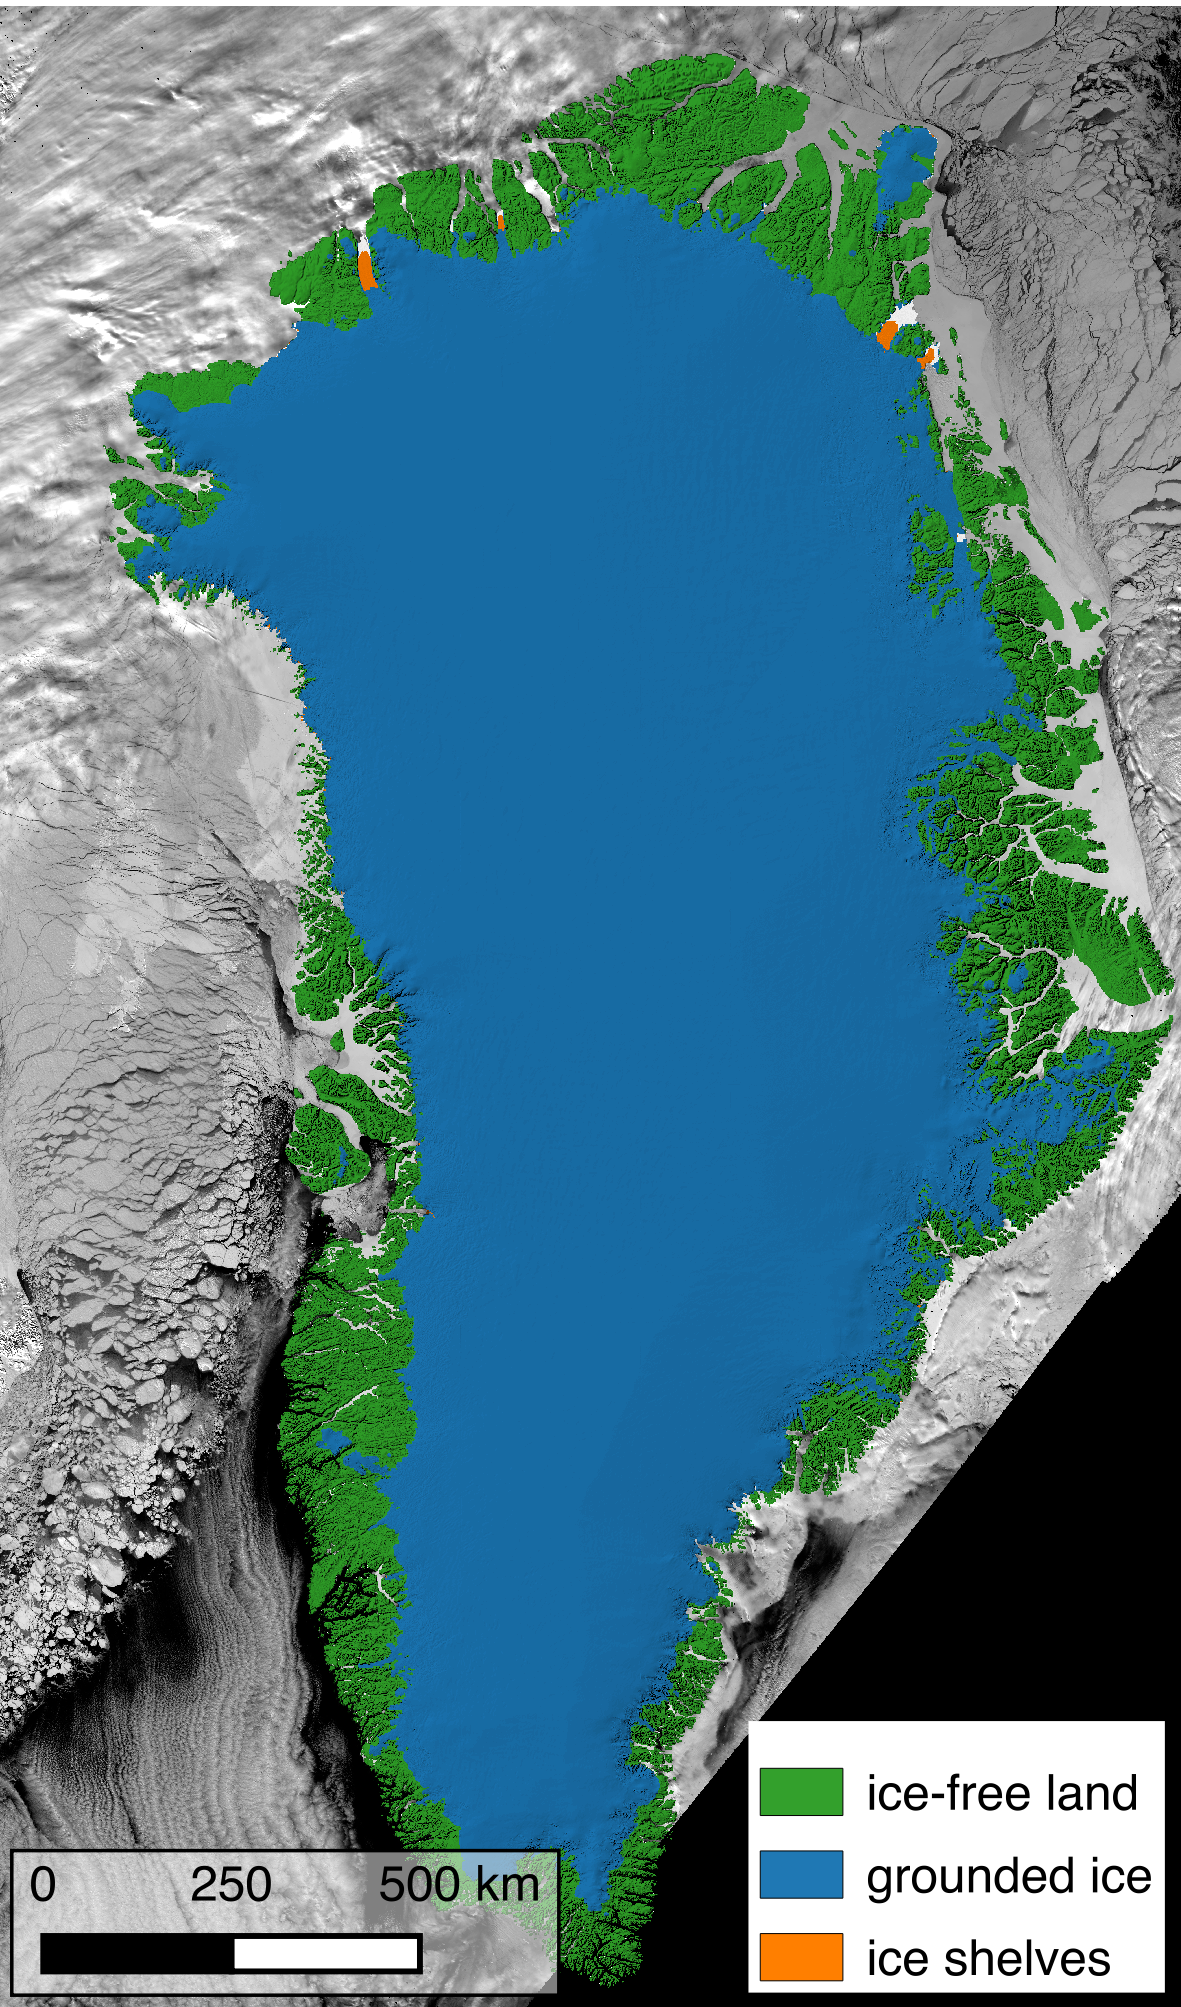
\includegraphics[height=0.8\textheight]{ice-mask-900m.png} \\ {\tiny \hfill PISM mask, by A.~Aschwanden}}
\includegraphics<2>[height=0.85\textheight]{jako-crop-mask-900m.png}
\only<3>{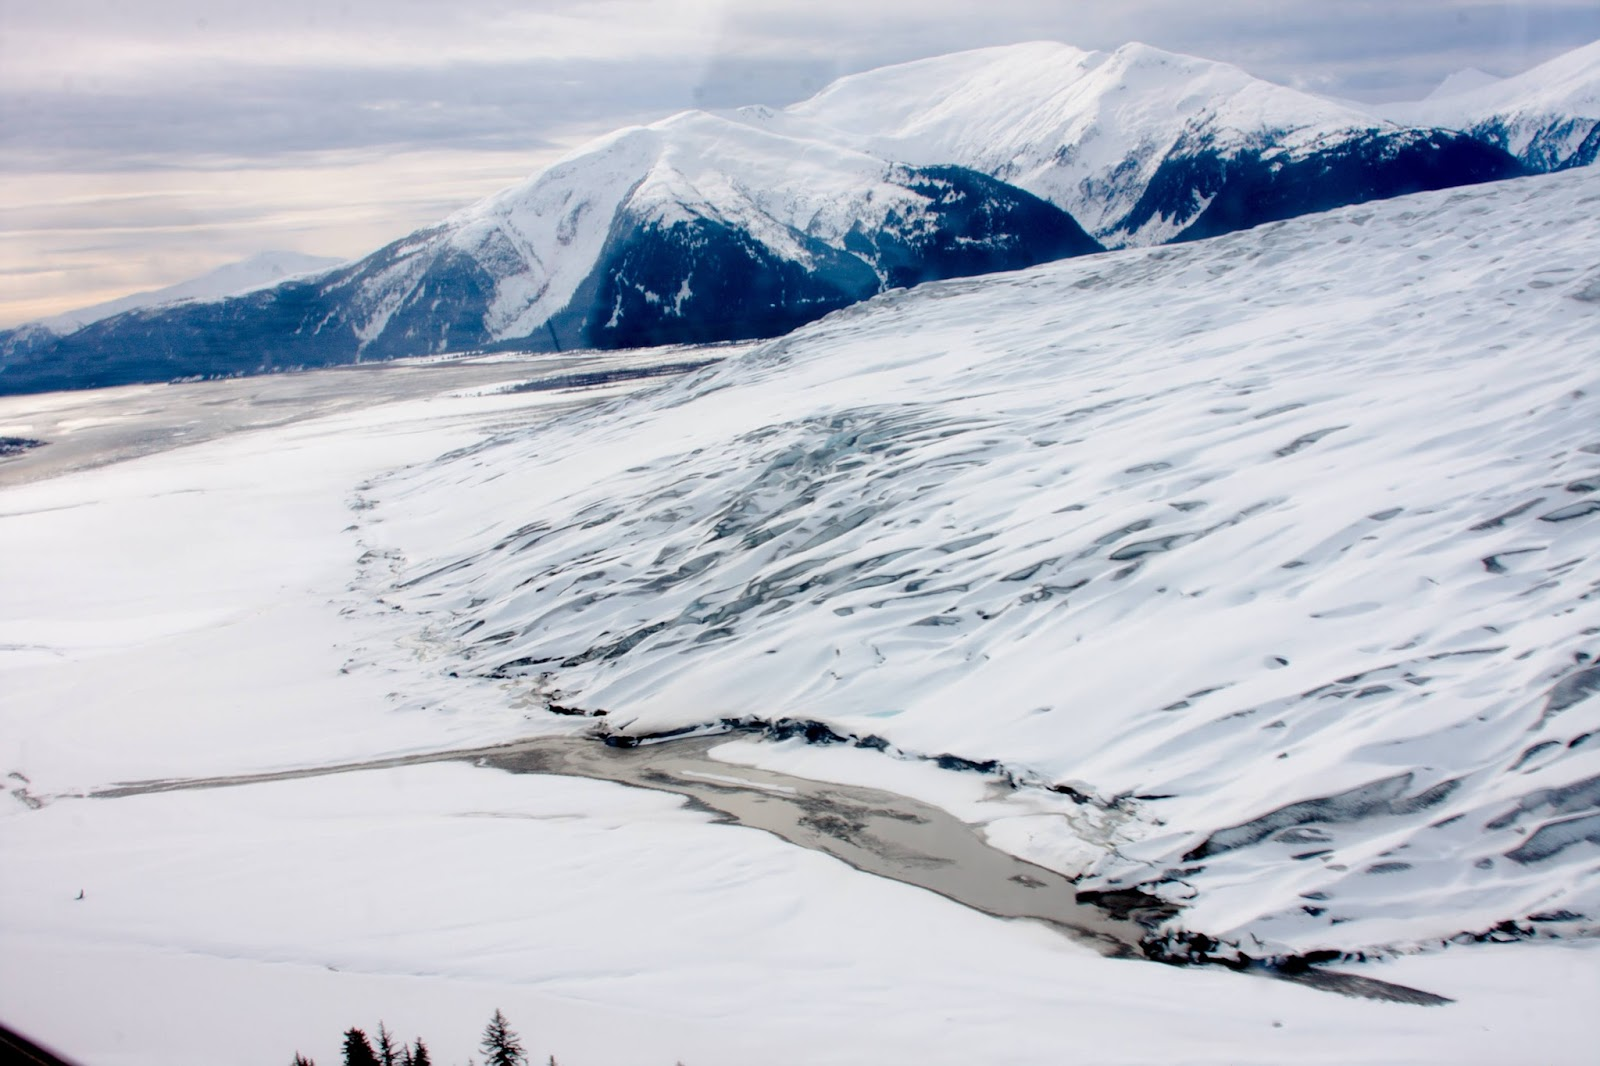
\includegraphics[width=1.05\textwidth]{truffertaku2016.jpg} \\ {\tiny \hfill Taku Glacier, Alaska, by M.~Truffer}}
\end{column}
\end{columns}
\end{frame}


\begin{frame}{computational goal: long-time, high-res runs}

\begin{itemize}
\item my goal:
\begin{quote}
\alert{routinely} simulate ice sheets on their natural time scales (ice age cycles \alert{$\gtrsim 10^5$ years}) at resolutions where bedrock bumps, outlet glaciers, ice streams, and grounding lines are resolved (\alert{$\lesssim 500$ m})
\end{quote}

\medskip
\scriptsize
\item PISM (Parallel Ice Sheet Model) not there yet \dots either long-time \emph{OR} high-res

\medskip
\normalsize
\item some concerns:
    \begin{enumerate}
    \item stress-balance solves expensive
        \begin{itemize}
        \item[$\circ$] if time steps are short then stress balance is a lot of work
        \item[$\circ$] \dots energy conservation (temperature and basal melt) too!
        \end{itemize}
    \item evolution of ice thickness $H(t,x,y)$ is diffusive \dots thus stiff
        \begin{itemize}
        \item[$\circ$] because ice flows downhill
        \end{itemize}
    \item ice margins are low-regularity
        \begin{itemize}
        \item[$\circ$] 2 reasons: (\emph{i}) constraint $H\ge 0$ and (\emph{ii}) degeneracy
        \end{itemize}
    \item bedrock is steep
    \end{enumerate}
\end{itemize}
\end{frame}


\begin{frame}{a performance model}

\begin{itemize}
\item grid spacing $h=\Delta x = \Delta y$ in 2D
    \begin{itemize}
    \item[$\circ$] (degrees of freedom) $=O(h^{-2})$
    \end{itemize}
\item time step limited by stability or accuracy:
    $$\Delta t \le O(h^q)$$

\vspace{-3mm}
    \begin{itemize}
    \item[$\circ$] $q=2$ for conditionally-stable explicit schemes on diffusions
    \item[$\circ$] accuracy alone suggests $0<q<1$ ? \dots a scientific question?
    \end{itemize}
\item solution at one time step:
    \begin{itemize}
    \item[$\circ$] $N(h)$ Newton iterations
    \item[$\circ$] $K(h)$ (preconditioned) Krylov steps per Newton
    \end{itemize}

\medskip
\item cost of computation on $\Omega \times [0,T]$:
\footnotesize
\begin{align*}
C(h) &= (\text{number of steps}) \cdot (\text{iterations per step}) \cdot (\text{cost of 1 residual}) \\
  &= O(h^{-q}) \cdot N(h) \cdot K(h) \cdot O(h^{-2})
\end{align*}
\normalsize

\vspace{-2mm}
    \begin{itemize}
    \item[$\circ$] explicit: $C(h) = O(h^{-2}) \cdot 1 \cdot 1 \cdot O(h^{-2}) = O(h^{-4})$ \hfill \alert{$\leftarrow$ beat this!}
    \end{itemize}
\end{itemize}
\end{frame}


\begin{frame}{ice sheet models}

\begin{itemize}
\item fixed computational domain $\Omega\subset \RR^2$ where inputs $b=$ (bed elevation) and $m=$ (mass balance) are given
    \begin{itemize}
    \item[$\circ$] \alert{$\Omega$ is only partly-covered by ice}
    \end{itemize}
\item shallow, possibly-hybrid, thickness-based \hfill {\scriptsize\color{Gray} $H,\, \mathbf{u}=(u,v)$}
        \begin{align*}
        H_t + \Div (-D \grad H + \bar{\mathbf{u}} H) &= m(x,t) && \text{mass conservation} \\
        \mathcal{L}(\mathbf{u},H) &= 0      && \text{shallow stress balance}
        \end{align*}
\item \emph{also}: Stokes, surface-elevation-based \hfill {\scriptsize\color{Gray} $s,\, \mathbf{u}=(u,v,w)$}
        \begin{align*}
        s_t + \mathbf{u}\big|_s \cdot (s_x,s_y,-1) &= m(x,t) && \text{surface kinematical} \\
        \Div \mathbf{u} &= 0            && \text{incompressibility} \\
        \mathcal{L}(\mathbf{u},s) &= 0  && \text{Stokes stress balance}
        \end{align*}
\item notation \& assumptions:
    \begin{itemize}
    \item[$\circ$] $H$ thickness, $s$ surface elevation, $\mathbf{u}$ velocity
    \item[$\circ$] $D=D(H,|\grad s|)$ is SIA diffusivity (nonlinear \& degenerate)
    \item[$\circ$] conservation of energy ignored for simplicity
    \item[$\circ$] Eulerian, fixed grid (structured or not)
    \end{itemize}
\end{itemize}
\end{frame}


\section{semi-discretizations}

\begin{frame}{semi-discretize in space}

\begin{itemize}
\item method of lines (MOL)
    \begin{itemize}
    \item[$\circ$] \emph{can you hand the thing to an ODE solver?}
    \end{itemize}
\item well-known: MOL for slow fluids is a DAE problem
\begin{align*}
\dot H &= f(H,\mathbf{u},t) && \text{mass conservation} \\
     0 &= g(H,\mathbf{u})   && \text{momentum conservation}
\end{align*}
\vspace{-5mm}
    \begin{itemize}
    \item[$\circ$] \emph{isn't implicit time-stepping required for DAEs anyway?}
    \end{itemize}
\item velocity variables only exist at positive-thickness locations $i$:
    $$\mathbf{u}_i \text{ exists } \quad \Longleftarrow \quad H_i > 0$$
\item thus ODE solver must handle \emph{events} like these?:
    \begin{itemize}
    \item[$\circ$] ice disappears during time step:  $H_i(t)>0 \to H_i(t+\Delta t)=0$
    \item[$\circ$] ice appears during time step:  $H_i(t)=0 \to H_i(t+\Delta t)>0$
    \end{itemize}
\end{itemize}
\end{frame}


\begin{frame}{MOL$+$events cannot scale}

\begin{center}
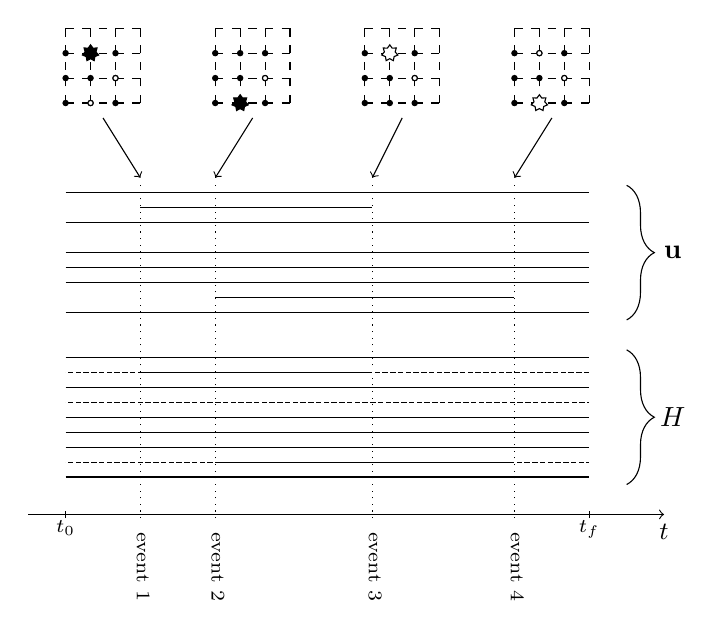
\begin{tikzpicture}[scale=0.95]
  %\draw[->,very thin] (-0.2,0.0) -- (1.2,0.0) node[below] {$x$};
  %\draw[very thin] (0.0,1.0) -- (0.0,0.0) -- (1.0,0.0);
  \pgfmathsetmacro\third{1.0/3.0}
  \pgfmathsetmacro\half{1.0/2.0}
  \pgfmathsetmacro\eps{0.001}

% time axis
  \draw[->,black,thin] (-0.5,-0.5) -- (8.0,-0.5) node[below] {\small $t$};
  \draw (0.0,-0.55) -- (0.0,-0.45) node[below] {\scriptsize $t_0$};
  \draw (7.0,-0.55) -- (7.0,-0.45) node[below] {\scriptsize $t_f$};

% events marked on time axis
  \draw[dotted] (1.0,-0.55) -- (1.0,3.9);
  \node[anchor=north, rotate=-90] at (1.25,-1.2) {\scriptsize event 1};
  \draw[dotted] (2.0,-0.55) -- (2.0,3.9);
  \node[anchor=north, rotate=-90] at (2.25,-1.2) {\scriptsize event 2};
  \draw[dotted] (4.1,-0.55) -- (4.1,3.9);
  \node[anchor=north, rotate=-90] at (4.35,-1.2) {\scriptsize event 3};
  \draw[dotted] (6.0,-0.55) -- (6.0,3.9);
  \node[anchor=north, rotate=-90] at (6.25,-1.2) {\scriptsize event 4};

% time-lines: H
  \foreach \y in {0,...,8} {
      \draw (0.0,\y * 0.2) -- (7.0,\y * 0.2);
  }
  \draw[white,dotted,thick] (0.0,1 * 0.2) -- (2.0,1 * 0.2);     % 1
  \draw[white,dotted,thick] (6.0,1 * 0.2) -- (7.0,1 * 0.2);     % 1
  \draw[white,dotted,thick] (0.0,5 * 0.2) -- (7.0,5 * 0.2);     % 5
  \draw[white,dotted,thick] (0.0,7 * 0.2) -- (1.0,7 * 0.2);     % 7
  \draw[white,dotted,thick] (4.1,7 * 0.2) -- (7.0,7 * 0.2);     % 7
  \draw [decorate,decoration={brace,amplitude=10pt,mirror}] (7.5,-0.1) -- (7.5,1.7) node [black,midway,right,xshift=0.3cm] {$H$};

% time-lines: u
  \pgfmathsetmacro\ushift{2.2}

  \foreach \y in {2,...,4} {
      \draw (0.0,\ushift + \y * 0.2) -- (7.0,\ushift + \y * 0.2);
  }
  \draw (0.0,\ushift + 0 * 0.2) -- (7.0,\ushift + 0 * 0.2);     % 0: full
  \draw (2.0,\ushift + 1 * 0.2) -- (6.0,\ushift + 1 * 0.2);     % 1
                                                                % 5: ice-free
  \draw (0.0,\ushift + 6 * 0.2) -- (7.0,\ushift + 6 * 0.2);     % 6: full
  \draw (1.0,\ushift + 7 * 0.2) -- (4.1,\ushift + 7 * 0.2);     % 7
  \draw (0.0,\ushift + 8 * 0.2) -- (7.0,\ushift + 8 * 0.2);     % 8: full
  \draw [decorate,decoration={brace,amplitude=10pt,mirror}] (7.5,\ushift+-0.1) -- (7.5,\ushift+1.7) node [black,midway,right,xshift=0.35cm] {$\mathbf{u}$};

% grids at events
  \pgfmathsetmacro\gshift{5.0}

  % t = 1.0, node 7 becomes icy
  \draw[xstep=\third,ystep=\third,black,thin,dashed] (0.0-\eps,\gshift+0.0-\eps) grid (1.0,\gshift+1.0);
  \foreach \x in {0,...,2} {
    \foreach \y in {0,...,2} {
        \filldraw (\x * \third,\gshift+\y * \third) circle (1.0pt);
    }
  }
  \node[draw,star,star points=7,fill=black,inner sep=0pt,minimum size=6.0pt] at (\third,\gshift+2 * \third) {};
  \fill[white] (\third,\gshift) circle (1.0pt);            % 1 ice-free
  \draw        (\third,\gshift) circle (1.0pt);
  \fill[white] (2 * \third,\gshift+\third) circle (1.0pt); % 5 ice-free
  \draw[]      (2 * \third,\gshift+\third) circle (1.0pt);
  \draw[->] (\half,\gshift-0.2) -- (1.0,\gshift-1.0);

  % t = 2.0, node 1 becomes icy
  \draw[xstep=\third,ystep=\third,black,thin,dashed] (2.0-\eps,\gshift+0.0-\eps) grid (3.0,\gshift+1.0);
  \foreach \x in {0,...,2} {
    \foreach \y in {0,...,2} {
        \filldraw (2.0 + \x * \third,\gshift+\y * \third) circle (1.0pt);
    }
  }
  \node[draw,star,star points=7,fill=black,inner sep=0pt,minimum size=6.0pt] at (2.0 + \third,\gshift) {};
  \fill[white] (2.0 + 2 * \third,\gshift+\third) circle (1.0pt); % 5 ice-free
  \draw[]      (2.0 + 2 * \third,\gshift+\third) circle (1.0pt);
  \draw[->] (2.0 + \half,\gshift-0.2) -- (2.0,\gshift-1.0);

  % t = 4.1, node 7 becomes ice free
  \draw[xstep=\third,ystep=\third,black,thin,dashed] (4.0-\eps,\gshift+0.0-\eps) grid (5.0,\gshift+1.0);
  \foreach \x in {0,...,2} {
    \foreach \y in {0,...,2} {
        \filldraw (4.0 + \x * \third,\gshift+\y * \third) circle (1.0pt);
    }
  }
  \node[draw,star,star points=7,fill=white,inner sep=0pt,minimum size=6.0pt] at (4.0 + \third,\gshift+2 * \third) {};
  \fill[white] (4.0 + 2 * \third,\gshift+\third) circle (1.0pt); % 5 ice-free
  \draw[]      (4.0 + 2 * \third,\gshift+\third) circle (1.0pt);
  \draw[->] (4.0 + \half,\gshift-0.2) -- (4.1,\gshift-1.0);

  % t = 6.0, node 1 becomes ice free
  \draw[xstep=\third,ystep=\third,black,thin,dashed] (6.0-\eps,\gshift+0.0-\eps) grid (7.0,\gshift+1.0);
  \foreach \x in {0,...,2} {
    \foreach \y in {0,...,2} {
        \filldraw (6.0 + \x * \third,\gshift+\y * \third) circle (1.0pt);
    }
  }
  \node[draw,star,star points=7,fill=white,inner sep=0pt,minimum size=6.0pt] at (6.0 + \third,\gshift) {};
  \fill[white] (6.0 + 2 * \third,\gshift+\third) circle (1.0pt); % 5 ice-free
  \draw[]      (6.0 + 2 * \third,\gshift+\third) circle (1.0pt);
  \fill[white] (6.0 + \third,\gshift+2*\third) circle (1.0pt); % 7 ice-free
  \draw[]      (6.0 + \third,\gshift+2*\third) circle (1.0pt);
  \draw[->] (6.0 + \half,\gshift-0.2) -- (6.0,\gshift-1.0);

\end{tikzpicture}


\end{center}

\vspace{-6mm}
\begin{itemize}
\item at each event the ice velocity dimension changes
\item ice sheet margins nearly fractal, so \emph{a lot} of events to handle
\item re-meshing at \emph{every} event probably won't scale
\end{itemize}
\end{frame}


\begin{frame}{semi-discretize in time}

\begin{itemize}
\item semi-discretize in time \emph{for understanding}
\item consider a single backward Euler time-step
    \begin{itemize}
    \item[$\circ$] better time-stepping later
    \end{itemize}
\item hybrid equations become (notation: $H=H_{\mathrm{new}}, \mathbf{u}=\mathbf{u}_{\mathrm{new}}$):
        \begin{align*}
        H - H_{\mathrm{old}} + \Delta t\, \Div (-D \grad H + \mathbf{u} H) &= \Delta t\, m \\
        \mathcal{L}(\mathbf{u},H) &= 0
        \end{align*}
\end{itemize}
\end{frame}


\begin{frame}{single time-step problem for mass conservation}

\small

\begin{itemize}
\item solve for $H$ \alert{subject to $H \ge 0$}:
        \begin{equation*}
        H - H_{\mathrm{old}} + \Delta t\, \Div \mathbf{q} = \Delta t\, m
        \end{equation*}
   \begin{itemize}

\vspace{-5mm}
   \item[$\circ$] where $\mathbf{q} = -D \grad H + \mathbf{u} H$
   \item[$\circ$] note: $D=D(H,|\grad s|) \to 0$ at margins
   \end{itemize}
\item make rigorous two ways:
    \begin{itemize}
    \item[$\circ$] variational inequality (VI)
    $$\int_\Omega (H - H_{\mathrm{old}} -\Delta t\, m) (\eta - H) - \Delta t\, \mathbf{q} \cdot \grad(\eta - H) \ge 0, \quad \forall \eta \ge 0$$
    \item[$\circ$] nonlinear complementarity problem (NCP)
\begin{align*}
F(H)   &= H - H_{\mathrm{old}} + \Delta t\,\Div \mathbf{q} - \Delta t\, m  \ge 0 \\
H      &\ge 0 \\
H F(H) &= 0
\end{align*}
    \end{itemize}
\end{itemize}
\end{frame}


\section{solving the equations for one time step}

\begin{frame}{solving the equations}
\begin{columns}
\begin{column}{0.55\textwidth}
\begin{itemize}
\item discretize in space:
    \begin{itemize}
    \item[$\circ$] e.g.~$M^\star=$ ($Q^1$ elements and \emph{finite volume} weak form ``$\int_V$'') Bueler 2016
    \end{itemize}
\end{itemize}
\end{column}
\begin{column}{0.45\textwidth}
\bigskip

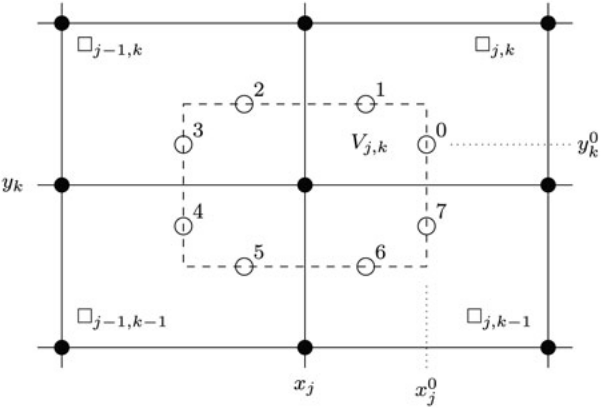
\includegraphics[width=\textwidth]{mstarstencil.png} 
\end{column}
\end{columns}

\medskip
\begin{itemize}
\item wrote small PETSc code for mass conservation problem:
    \begin{itemize}
    \item[$\circ$] MOL using $M^\star$
    \item[$\circ$] tells \texttt{TS} object which part is stiff: $F(H_t,H) = G(t,H)$
        \begin{itemize}
        \item  $F=H_t + \Div \mathbf{q}$ and $G=m$
        \end{itemize}
    \item[$\circ$] allows any implicit or IMEX time-stepping
    \end{itemize}
\item equations at each time step are solved with
    \begin{itemize}
    \item[$\circ$] NCP-adapted (``reduced-space'' or ``semi-smooth'') Newton
        \begin{itemize}
        \item[$\ast$] \texttt{-snes\_type vinewton\{rs|ss\}ls} \hfill \tiny Benson \& Munson 2006 \normalsize
        \end{itemize}
    \item[$\circ$] + Krylov solver + preconditioning
    \end{itemize}
\end{itemize}
\end{frame}


\begin{frame}{margin advance experiment: Newton iterations}

\begin{columns}
\begin{column}{0.45\textwidth}
\begin{itemize}
\item consider a single 10-year \texttt{beuler} time step
\item of a Greenland-sized radial ice sheet
    \begin{itemize}
    \item[$\circ$] flat bed, $m=0$
    \item[$\circ$] margin advance 975 m
    \end{itemize}
\item reduced-space Newton solver sees Jacobian in inactive variables only
    \begin{itemize}
    \item[$\circ$] states are admissible
    \item[$\circ$] dimension changes at each Newton step
    \end{itemize}
\item<2> on fine grids ($\lesssim 1$ km) the number of Newton iterations is proportional to margin motion divided by $\Delta x$
\end{itemize}\end{column}
\begin{column}{0.55\textwidth}

\bigskip
\hfill 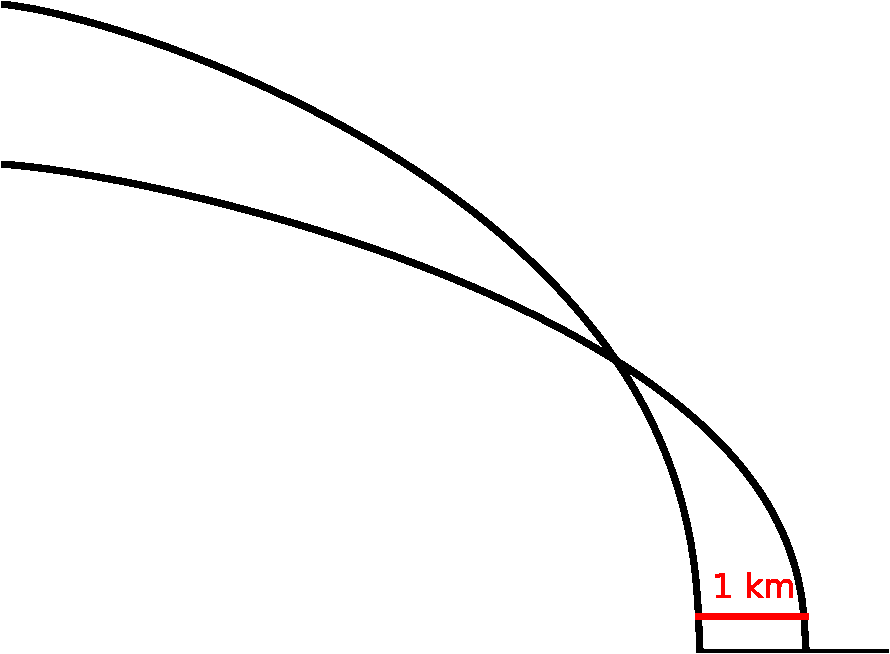
\includegraphics[width=0.7\textwidth]{halfarcartoon.pdf}

\bigskip
\includegraphics<1>[width=\textwidth]{newtoniters.pdf}
\includegraphics<2>[width=\textwidth]{newtonitersFIT.pdf}
\end{column}
\end{columns}
\end{frame}


\begin{frame}[fragile]
\frametitle{margin advance experiment: preconditioners}
\begin{itemize}
\item fixed MPI rank = 64
\item compare preconditioners:

\small
\centerline{\texttt{-snes\_type vinewtonrsls -ksp\_type gmres -pc\_type X}}
\normalsize
\item Krylov iterations per Newton step:
\end{itemize}

\begin{center}
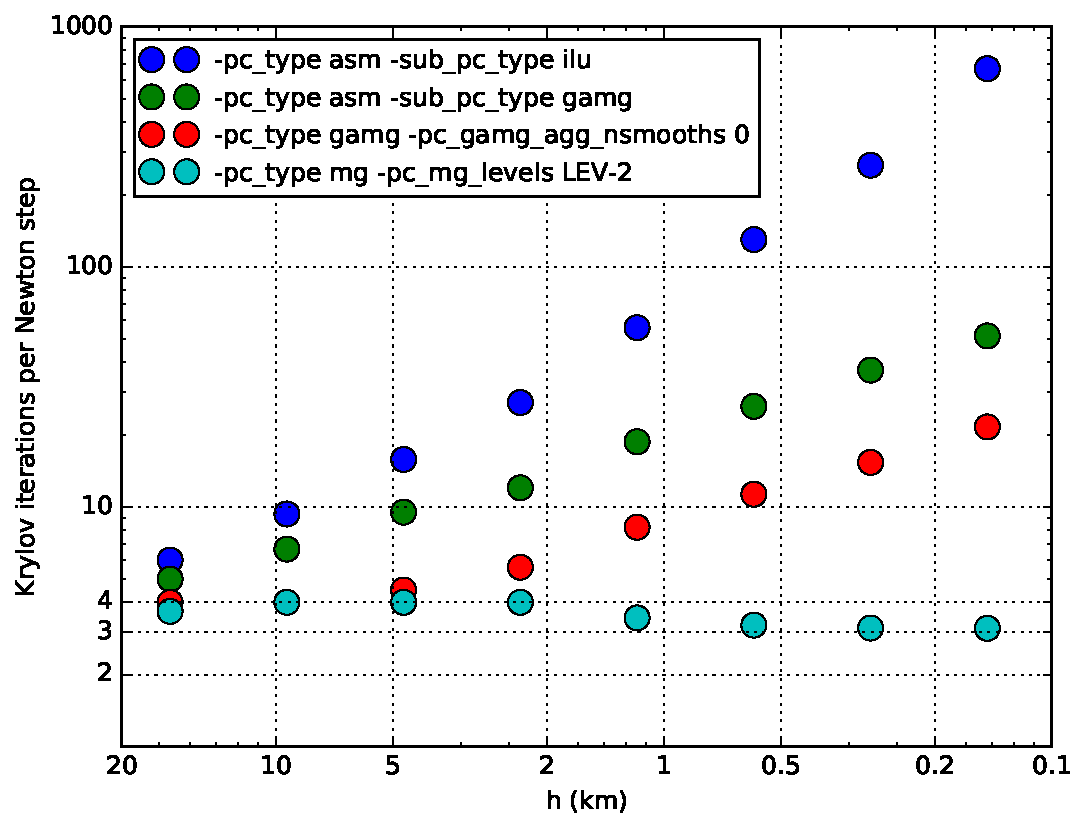
\includegraphics[width=0.75\textwidth]{pcksppernewton.pdf}
\end{center}
\end{frame}


\begin{frame}{margin advance experiment:  weak scaling?}
\begin{itemize}
\item very preliminary weak-scaling evidence
    \begin{itemize}
    \item[$\circ$] ranks $1,4,16,64$
    \item[$\circ$] fixed d.o.f.~per process: $2.4 \times 10^6$
    \item[$\circ$] \texttt{-pc\_type mg}
    \end{itemize}
\item time per Newton step: \hfill \dots \emph{should be flat!}

\begin{center}
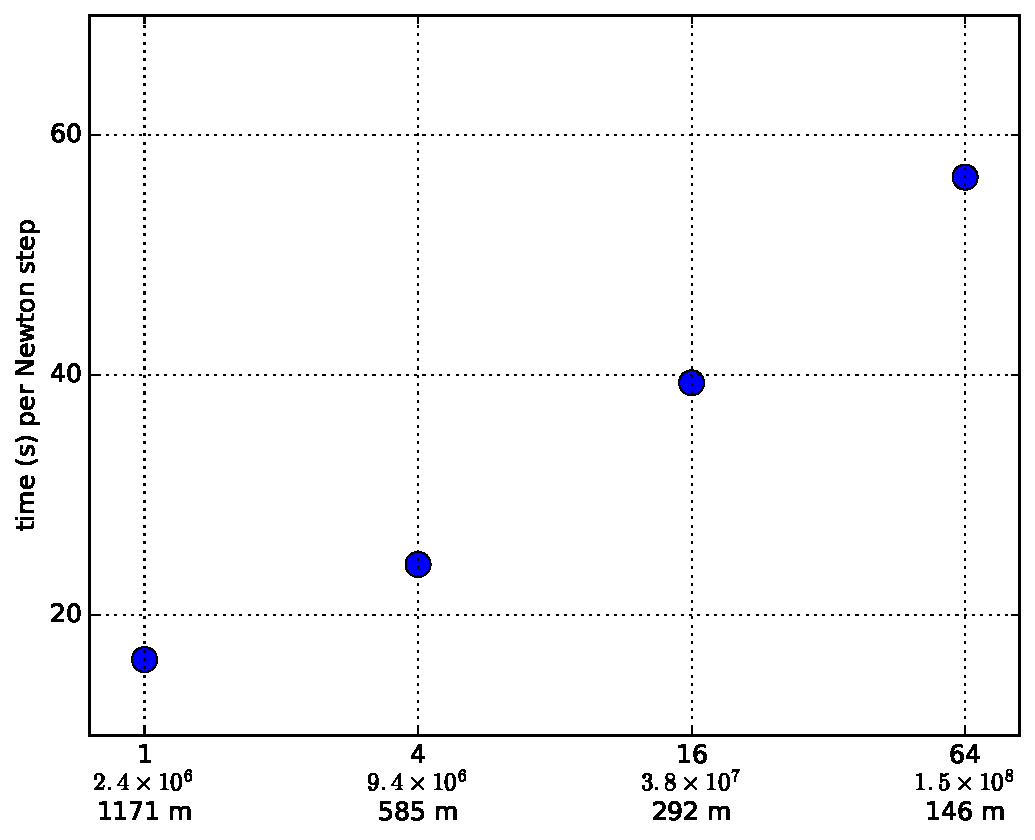
\includegraphics[width=0.5\textwidth]{timepernewtonweak.pdf}
\end{center}

\item<2> the good news: $\Delta t/\Delta t_{FE} = 9 \times 10^4$ on finest grid
\end{itemize}
\end{frame}


\section{some early results}

\begin{frame}{example: 50ka run with topography and sliding}
\begin{center}
% use  mogrify -trim *.png
\mbox{$t=0$ a 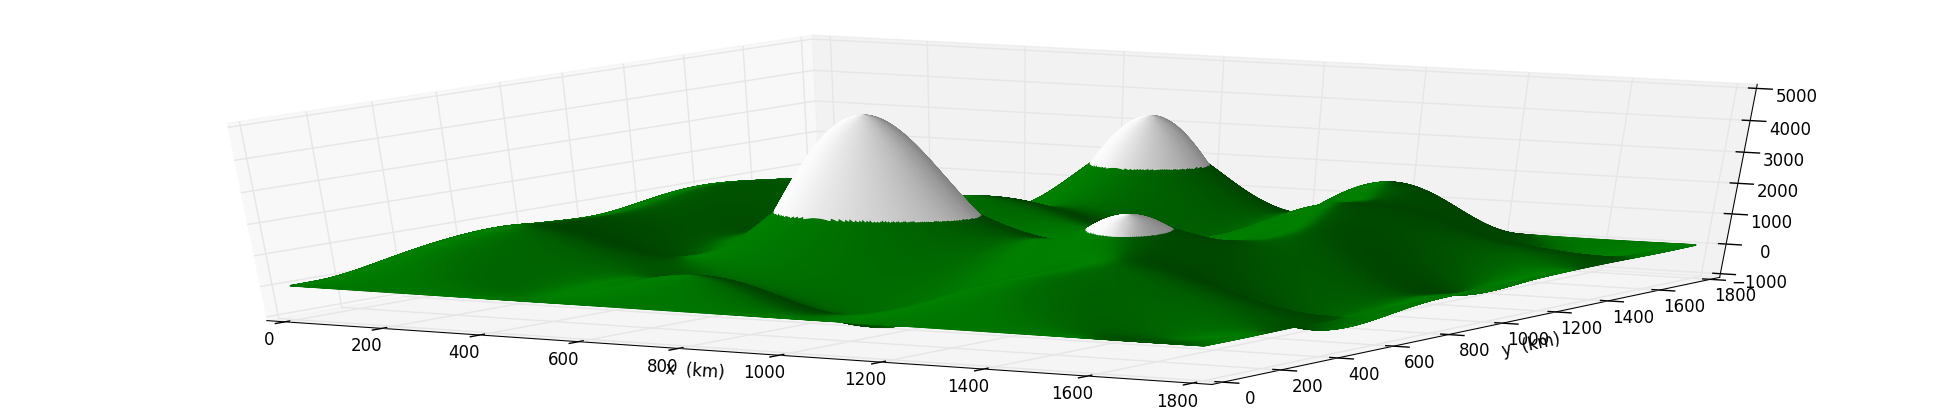
\includegraphics[height=0.25\textheight]{startsheet.png}}

\mbox{$t=50$ ka 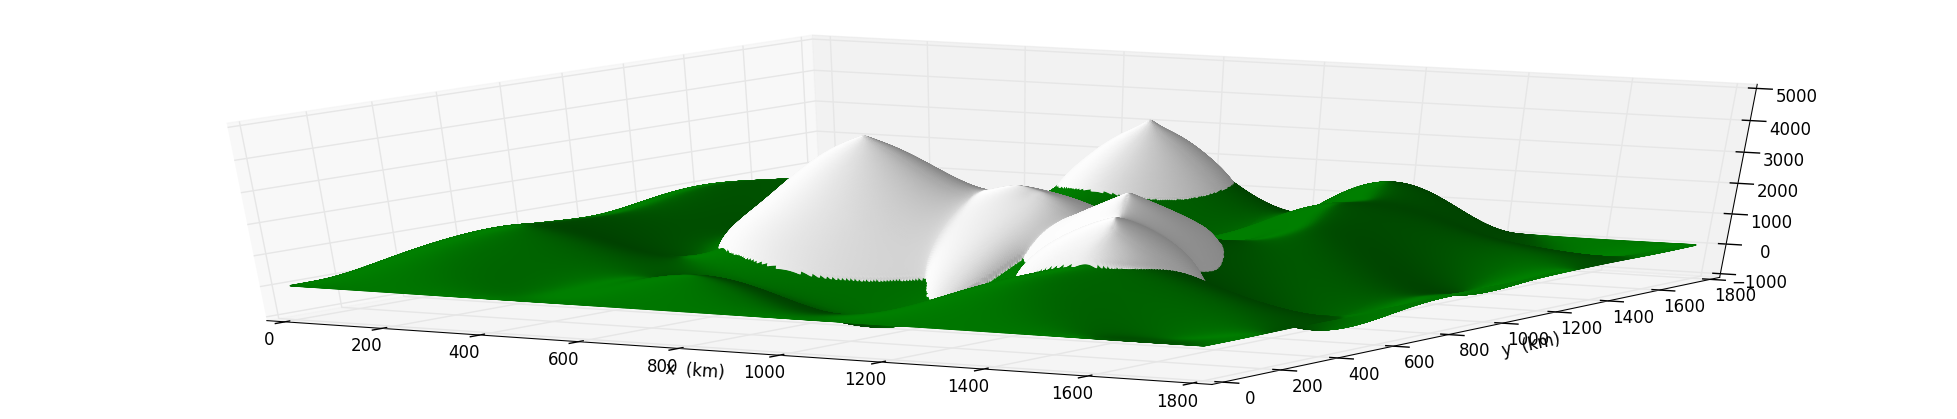
\includegraphics[height=0.25\textheight]{endsheet.png}}
\end{center}

\begin{itemize}
\item solve: $H_t + \Div \mathbf{q} = m$ where $\mathbf{q} = -D\grad H + \mathbf{u} H$
    \begin{itemize}
    \item[$\circ$] imposed ``sliding'' $\mathbf{u}(x,y)$
    \item[$\circ$] elevation-dependent accumulation/ablation $m=m(s)$
    \end{itemize}
\end{itemize}
\end{frame}


\begin{frame}{50ka run: time-stepping performance}
\begin{itemize}
\item ARKIMEX(3): adaptive Runge-Kutta implicit/explicit 3rd-order (3 stage) time-stepping
\item at least three nonlinear solves per time step
\end{itemize}
\begin{center}
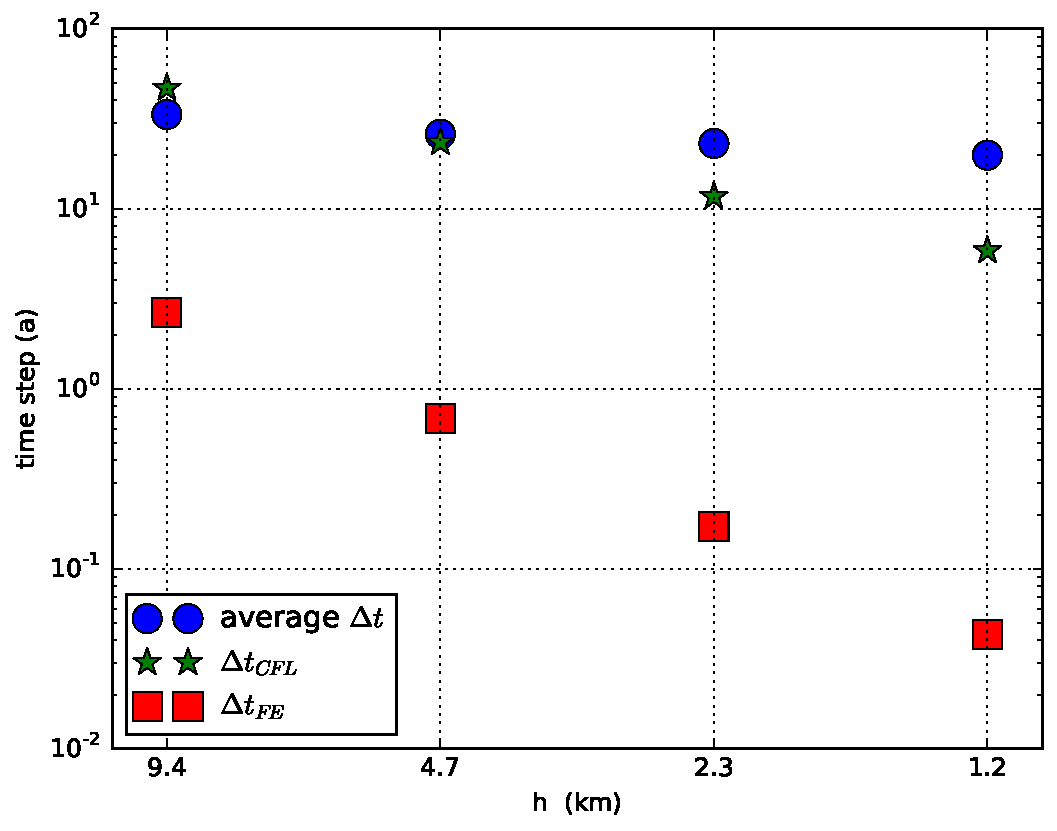
\includegraphics[width=0.75\textwidth]{dtfiftyka.pdf}
\end{center}
\end{frame}


\begin{frame}{example: Greenland ice sheet $\Delta t=\infty$}

\begin{columns}
\begin{column}{0.5\textwidth}
\begin{itemize}
\item steady geometry $H(x,y)$ of the Greenland ice sheet
  \begin{itemize}
  \item[$\circ$] given $m(x,y)$ and $b(x,y)$
  \end{itemize}
\item<1-2> Bueler 2016, J.~Glaciol.
\item<1> one $\Delta t=\infty$ step
  \begin{itemize}
  \item[$\circ$] 900 m structured grid
  \item[$\circ$] $7\times 10^6$ d.o.f.
  \end{itemize}

\bigskip
\item<2> \emph{but} Newton convergence suffers from bed roughness
\end{itemize}
\end{column}
\begin{column}{0.5\textwidth}
\only<1>{\hfill 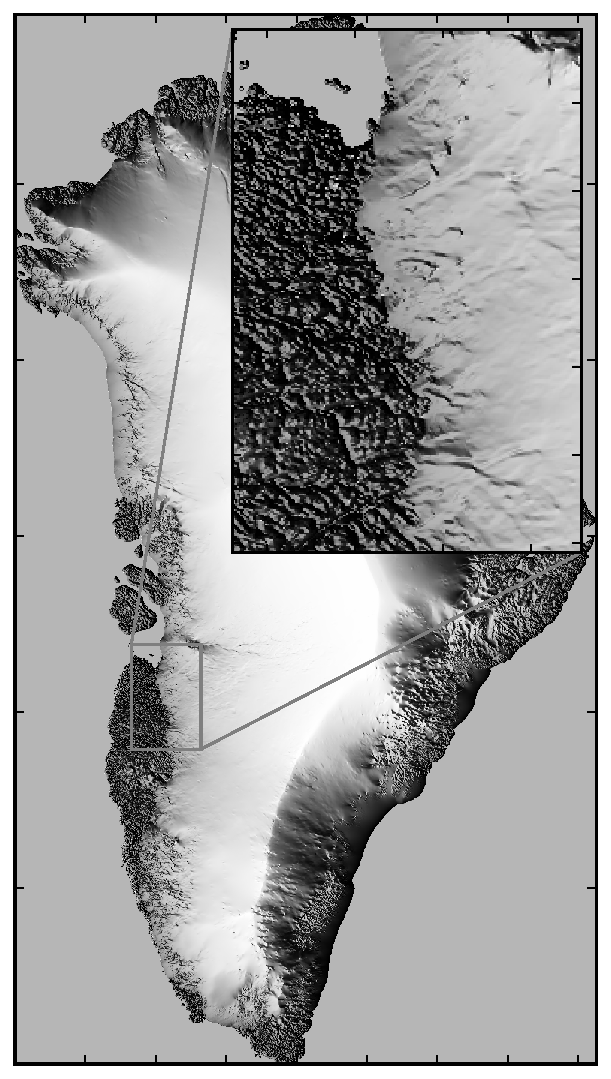
\includegraphics[height=0.8\textheight]{grnwinset.pdf}}

\includegraphics<2>[width=\textwidth]{rseps.pdf}
\end{column}
\end{columns}
\end{frame}




\begin{frame}[fragile]
\frametitle{summary}
\begin{itemize}
\item recommendations for implicit time-stepping of thickness-based mass conservation:
  \begin{itemize}
  \item[$\circ$] enforce $H\ge 0$ as NCP or VI
  \item[$\circ$] use reduced-space solver which has admissible states for stress balance solution
  \item[$\circ$] use geometric multigrid (?)
  \item[$\circ$] result: $>10^5 \,\Delta t_{\text{FE}}$ achievable
  \end{itemize}
\item some limitations:
  \begin{itemize}
  \item[$\circ$] extra Newton steps needed to move margins $x$ grid spaces
  \item[$\circ$] bed roughness eventually limits Newton solver convergence
  \item[$\circ$] calving and front-melting not addressed in this framework \dots yet
  \end{itemize}

\bigskip
\item wiser now? \dots if I were to start over with PISM:
\scriptsize
\begin{verbatim}
mpiexec -n N newpism -da_refine M \
   -ts_type arkimex -snes_type vinewtonrsls -pc_type mg
\end{verbatim}
\end{itemize}
\end{frame}


\end{document}
